\documentclass{sigchi}

% Remove or comment out these two lines for final version
\toappearbox{\Large Submitted to CHI'13. \\Do not cite, do not circulate.}
\pagenumbering{arabic}% Arabic page numbers for submission. 

% Use \toappear{...} to override the default ACM copyright statement (e.g. for preprints).

% Load basic packages
\usepackage{balance}  % to better equalize the last page
\usepackage{graphicx} % for EPS, load graphicx instead
\usepackage{times}    % comment if you want LaTeX's default font
\usepackage{url}      % llt: nicely formatted URLs
\usepackage{tabularx}

% llt: Define a global style for URLs, rather that the default one
\makeatletter
\def\url@leostyle{%
  \@ifundefined{selectfont}{\def\UrlFont{\sf}}{\def\UrlFont{\small\bf\ttfamily}}}
\makeatother
\urlstyle{leo}


% To make various LaTeX processors do the right thing with page size.
\def\pprw{8.5in}
\def\pprh{11in}
\special{papersize=\pprw,\pprh}
\setlength{\paperwidth}{\pprw}
\setlength{\paperheight}{\pprh}
\setlength{\pdfpagewidth}{\pprw}
\setlength{\pdfpageheight}{\pprh}

% Make sure hyperref comes last of your loaded packages, 
% to give it a fighting chance of not being over-written, 
% since its job is to redefine many LaTeX commands.
\usepackage[pdftex]{hyperref}
\hypersetup{
pdftitle={SIGCHI Conference Proceedings Format},
pdfauthor={LaTeX},
pdfkeywords={SIGCHI, proceedings, archival format},
bookmarksnumbered,
pdfstartview={FitH},
colorlinks,
citecolor=black,
filecolor=black,
linkcolor=black,
urlcolor=black,
breaklinks=true,
}

% create a shortcut to typeset table headings
\newcommand\tabhead[1]{\small\textbf{#1}}


% End of preamble. Here it comes the document.
\begin{document}

\title{Touch keyboard hierarchical spatial models with back-offs for personal 
and hand posture adaptation}

% Note that submissions are blind, so author information should be omitted
\numberofauthors{3}
\author{
  \alignauthor 1st Author Name\\
    \affaddr{Affiliation}\\
    \affaddr{Address}\\
    \email{e-mail address}\\
  \alignauthor 2nd Author Name\\
    \affaddr{Affiliation}\\
    \affaddr{Address}\\
    \email{e-mail address}\\
  \alignauthor 3rd Author Name\\
    \affaddr{Affiliation}\\
    \affaddr{Address}\\
    \email{e-mail address}\\
}

% Teaser figure can go here
%\teaser{
%  \centering
%  \includegraphics{Figure1}
%  \caption{Teaser Image}
%  \label{fig:teaser}
%}

\maketitle

\begin{abstract}
In this sample paper, Sheridan Printing Co., Inc. 
describe the formatting requirements for
SIGCHI Conference Proceedings, and this sample file
offers recommendations on writing for the worldwide
SIGCHI readership. Please review this document even if
you have submitted to SIGCHI conferences before, some
format details have changed relative to previous years.
\end{abstract}

\keywords{
	Guides; instructions; author's kit; conference publications;
	keywords should be separated by a semi-colon.
	\\\textcolor{red}{Mandatory section to be included in your final version.}
}

\category{H.5.m.}{Information Interfaces and Presentation (e.g. HCI)}{Miscellaneous
\\
\textcolor{red}{See: \url{http://www.acm.org/about/class/1998/}
for more information and the full list of ACM classifiers and descriptors. 
Mandatory section: On the submission page
only the classifiers' letter-number combination will need to be entered.}
}

\terms{
	Human Factors; Design; Measurement. 
	If you choose more than one ACM General Term, 
	separate the terms with a semi-colon.
\\
\textcolor{red}{If you choose more than one ACM General Term, 
separate the terms with a semi-colon. See list of ACM terms at:
\url{http://www.sheridanprinting.com/sigchi/generalterms.htm}.
Optional section to be included in your final version.}
}

\section{Introduction}
Modern touch screen keyboards are error-tolerant. They can correct sloppy touch
events to user intended words based on a combination of language model predictions and a spatial model estimation. 
The spatial model that converts a touch point into the probabilities of keys depends on a number factors: hand-posture (e.g. two thumbs vs. one finger [1]), the individual [2] and the target key’s position [1].

In this paper we explore different ways of touch screen keyboard adaptation and
their effects in key detection accuracy and auto-correction with language
models.

 1. Spatial model building
2. Hand-posture classifier
3. User adaptation
4. Key detection process

\section{Related work}


The prior work from Findlater et al. [2] suggests that personalized touch keyboard which adapts its underlying key-press classification models to the users can improve typing speed.  But they assume that the same individual would maintain the same hand posture. 

We observe that the same individual may change hand posture even on the same device. The study from Azenkot and Zhai [1] shows that there are significant differences in typing speed and error rate between two-thumb input posture and one-finger input posture. More importantly, the horizontal and vertical offsets are different for each key and posture combinations. This suggests that automatic posture detection and posture adaptive spatial model can potentially improve key detection accuracy.

When the user switches hand posture, the adapted spatial model may in fact give less accurate estimations in the transient period of adaptation. To mitigate this problem and consider all the different facets of adaptation, we designed a hierarchical spatial models with back-offs for touch keyboards.  

Our approach consists the following components:

\section{Hierarchical Adaptive Spatial Models}

To incorporate different strategies of adaptations, we propose a hierarchical
spatial model consisting of a large number of sub-models.
The entire model can be viewed as a hierarchy of sub-models in different
“orders” (Figure. \ref{fig:hierarchy}).

\begin{figure}[tb]
  \centering
  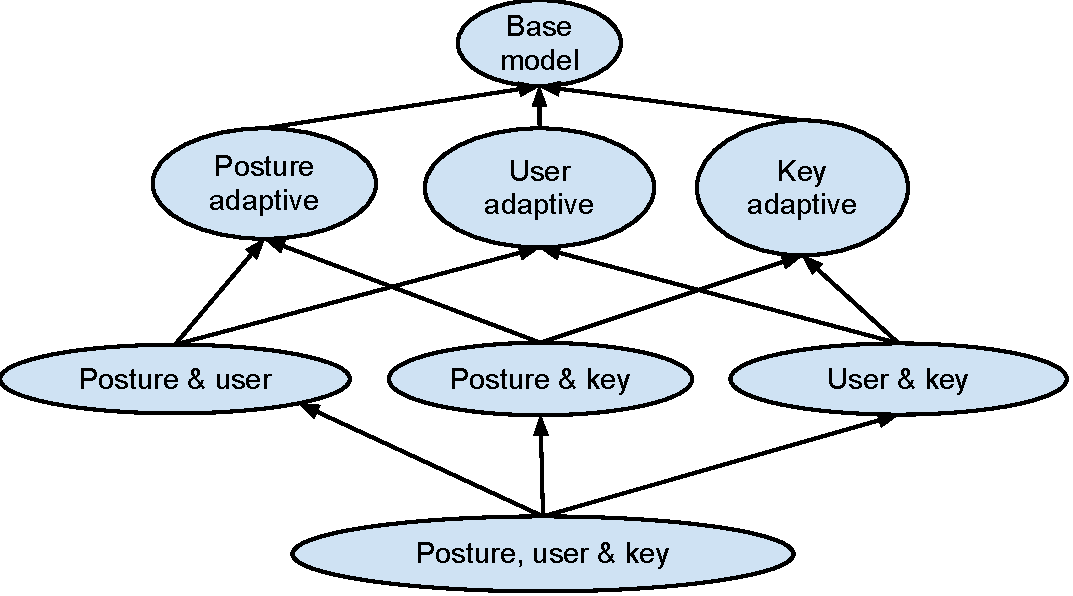
\includegraphics[width=1\columnwidth]{figures/hierarchical-spatial-model.pdf}
  \caption{Hierarchical spatial models}
  \label{fig:hierarchy}
\end{figure}

The zeroth order is the base model which is key, person, and posture
independent. This is the most general model combining all data together. The
higher order models consist of a combination of spatial models that adapt to hand posture (e.g. one finger, two thumbs, or ten fingers on tablets) , key or bi-letters (e.g. "h/t” where the current target letter is the “h” key and the previous letter is “t”), and the individual user. Each combination of the conditions needs sufficient number of samples to build a reliable model. Each such sub-model would only become active when its reliability passes a set threshold (e.g.100+ points had been collected). otherwise these models that are still “growing” but in “dormant” mode.

We compare key detection accuracy with different models to analyze their relative effectiveness (Table 2). This can inform us the order of the back-off models to use when there is not enough data for higher order models. 10-fold cross validation is used, and all left-handed users (3 out of are removed.The training and testing data sets have different sets of users.
Evaluation is based on a data set collected from an earlier study of 32
participants. The details of the study can be found in this paper \cite{}. 
(Briefly describe the data set.)

The simpliest detection method is checking whether a given tapping point is
with a certain key bound. The base model has 0 x and y offsets and the same
spherical covariance matrix for all the keys. Key detection based on this model is essentially choosing the key that has the shortest Euclidean distance from the tapping coordinates.

A basic key adaptive model is building a bivariate Gaussian model for each key using data from many different users. Then the key detection process involves choosing the key whose Gaussian model gives the highest probability for the given (x, y) tapping coordinates. When this is combined with posture and individual adaptation, more specialized Gaussian models are built for each key.

The difference in key detection accuracy between using the base model only and
the key adaptive model is not big. It is even surprising that key adaptive model
gives slightly lower accuracy. and tested on different sets of users.
Since the key adaptive model can be trained offline by collecting data from a large number of users, this shows that it can be used as the basic backup model once we collect enough data. The user and key adaptive model gives much higher accuracy than the posture and key adaptive model. This suggests that user and key adaptation can have higher priority. Only when we do not have enough data for the user, we can use posture and key adaptation.

\begin{table} [tb]
  \centering
  \begin{tabular*}{0.5\textwidth}{ | l | c | }
    \hline
    Key bound check & 91.382 \\
    \hline
    Distance from the center of the keys & 92.024 \\
    \hline
    Base model (same Gaussian model for all the keys) & 92.147 \\
    \hline
    Key adaptive model  & 91.977 \\
    \hline
    Posture and key adaptive & 92.942 \\
    \hline
    User and key adaptive   & 93.155 \\
    \hline
  \end{tabular*}
  \caption{Comparison of key detection accuracy (no language model) with
  different spatial models using 10-fold cross validation.}
  \label{tab:comparison}
\end{table}


For posture and key adaptation, there are 13.25% and 2.24% reduction in error rates compared to key adaptation only for the Pepper and Salt data sets respectively. Two postures are considered here: one finger versus two thumbs. The accuracy is based on perfect knowledge of the posture which represents an upper bound for posture adaptation for these data sets. In the actual implementation, the posture model can be turned on when we have high enough confidence about the posture classification.

For user & key adaptation, for each fold, we use 90% of the users to train the combined back-off key models. Then for each of the 10% testing users,  a fraction k of the data for each key is used to train the user adaptive key models. The accuracy of these data points are tested on the combined key models. The remaining 50% of the data for each user are tested on the user adaptive models together with the combined model for backup. The backup is used when there is not enough data for certain key (we used 10 data points) to build the Gaussian model. For the Pepper data set, k is set to be 50%; and for the Salt data set, k is set to be 70%. This is because Pepper data set has larger number of data points per subject (2634 data points / subject) versus that in the Salt data set (777 data points / user).

The key spatial model can also be more specialized to include bi-letter patterns that occur frequently, for instances, h followed by e, t followed by h etc. Figure 2 shows the (x, y) coordinates of the tapping points for letter “e” from one of our data sets, and the 0.95 confidence ellipses of the Gaussian models for different conditions. The plot shows that when we combine data for all the posture together, the distribution of points for “e” after “h” is very slightly different from that of all “e”. But if we look at “e” after “h” for one-finger input (cyan color), the difference is bigger. Another point to note is that, since these are highly frequent patterns, even a small improvement in detecting these keys based on these more specialized models may give a bigger improvement in the overall key detection accuracy. 


Figure 2. Comparison of Gaussian models (0.95 confidence ellipses) for letter “e”

\section{Input hand posture adaptation}
To incorporate posture adaptive spatial models, we need to develop a method to
detect users' posture when they are typing on the touch screens. 

2. Hand-posture classifier

We developed a hand-posture classifier that constantly returns an estimate of the user’s current posture (two thumbs vs. one finger input).

The analysis of variance based on the tapping coordinates for each key collected from 32 participants shows that, for different postures, there are significant differences in the means of the x coordinate for the keys on the left side of the keyboard and the "space” key (p < 0.05). For the y coordinate, the difference for different postures is significant for the “l”, “m” and “p” keys. This shows that posture adaptation can help with the key detection accuracy.

Our method of hand-posture classification is based on Fitts’ law which states that the time (T) required to move to a target is a function of the distance (D) to the target and the size (W) of the target (Equation 1).
T=a+blog2(1+DW)                                                  (1)
The insight here is that we expect the one-finger input posture follows this law,  but two-thumbs input may not. For example, when the user types “al”, it takes longer time to type using one finger because the distance between these two keys are large, but with two thumb, it can be very fast because she can use the left thumb to type “a” and the right thumb for “l”.
Figure 3. Tapping points data from input on a Galaxy Nexus phone

Figure. 3 shows the relationship between the time elapsed  and the log distance travelled between consecutive key presses. We can see that for the one-finger input (green points), the time takes increases with distance whereas for the two-thumb input, there is no obvious trend. The difference is more significant when the log distance (natural log) is greater than 5 px.

Based on this finding, we include the time elapsed and the log distance between two consecutive key presses as the features for the posture classifier. To account for individual typing speed differences, we also use normalized time elapsed between consecutive key presses as the third feature. It is calculated according the following equation:
Normalized time elapsed = time elapsed / average time elapsed for the last 10 key presses

We train a SVM classifier with these 3 features for consecutive tap points that are on different sides of the keyboard and whose log distance is at least 5 px. Table 1 shows the classification accuracies for 3 data sets. For each data set, 70% of the data is used for training and 30% of the data is used for testing. The users in the training and testing data sets are different.

The Pepper (84292 filtered data points) and Salt (30308 aligned and filtered data points) data sets we use consist tapping points from different users with different postures. Users were asked to enter specific phrases or repeated words. For the Pepper data set, users typed slowly and more precisely in general while for the Salt data sets, users were instructed to type fast and naturally.
Pepper data set (phrases) Salt data set (phrases)
Single tap classification accuracy for keys with previous key on the different side of the keyboard 83.559% (11090/13272) 78.693% (4288/5449)
Classification with a sliding time window 87.894% (27299/31059) 80.427% (9332/11603)

Table 1. Posture classification result 

The single tap classifier gives probability scores for the two postures for key taps whose previous key tap is on the different side of the keyboard. For the rest of the key taps, the scores for both postures are 0. In order to classify every key tap and assuming the user does not change posture rapidly, we look at a sliding time window of 10 key taps (about 2 words). For each time window, we use another SVM classifier with the following features:
Correlation between time elapsed and log distance (this feature has the advantage of being speed independent) (see Figure. 4).
The average probability score for each tap to be one-finger input.
The average probability score for each tap to be two-thumb input.
The average number of taps classified as one-finger input.
The average number of taps classified as two-thumb input.
The sliding time window classifier also gives probability scores for each posture.

The second row of Table 1 shows the overall classification accuracy for each key tap in the test data set. Because of the sliding window approach, the posture for the first 10 key taps for each new session is unknown, and we can use a lower order spatial model in this case. Also we can turn on the posture adaptive spatial model only when the probability score for one posture is much higher than the other. 
Figure. 4 Correlation between time elapsed and log distance between consecutive 
key presses for every 10 keys. There is a stronger correlation for one- 
finger input than that for two-thumb input
3. User adaptation

Fig. 5  A look at how key detection accuracy changes as the number of tapping points used for building the user adaptive Gaussian model for key ‘E’ increases
4. Key detection process 

In the decoding process, a higher order more specialized model is used if it meets a set of conditions such as a particular posture mode is detected with high confidence and the corresponding model (e.g. h/t, one-finger) is available (live, matured). Otherwise we back off to a lower order model, all the way to a base model which is key, individual and posture independent if necessary.

\section{Implementation and off-device simulation}
\begin{table}[tb]
  \centering
  \begin{tabularx}{\columnwidth}{|X|c|}
  \hline
  Spherical cov & 91.307\% \\
  \hline
  Learned covariance & 91.359 \\
  \hline
  Key adaptive  & 91.292 \\
  Posture and key adaptive  & 91.598 \\
  User and key adaptive & 91.7438 \\
  User and key adaptive (combine user and population Gaussian)  & 91.486\% \\
  User and key adaptive (combine user and population, distance only) &  92.700\%
  \\
  \end{tabularx}
  \caption{Off device simulation result}
  \label{tab:off-device}
\end{table}


(With language model result)

1. Azenkot, S.,  Zhai, S. (2012). Touch Behavior with Different Postures on Soft Smart Phone Keyboards. In Proceedings of MobileHCI (MobileHCI '12). To appear.

2. Findlater, L., Wobbrock, J.O. (2012). Personalized input: improving ten-finger touchscreen typing through automatic adaptation. Proc. SIGCHI Conference on Human Factors in Computing Systems (CHI 2012), 815-824.
\section{Conclusion}

It is important that you write for the SIGCHI audience.  Please read
previous years' Proceedings to understand the writing style and
conventions that successful authors have used.  It is particularly
important that you state clearly what you have done, not merely what
you plan to do, and explain how your work is different from previously
published work, i.e., what is the unique contribution that your work
makes to the field?  Please consider what the reader will learn from
your submission, and how they will find your work useful.  If you
write with these questions in mind, your work is more likely to be
successful, both in being accepted into the Conference, and in
influencing the work of our field.

\section{Acknowledgments}

We thank all the volunteers, and all publications support
and staff, who wrote and provided helpful comments on previous
versions of this document.  Some of the references cited in this paper
are included for illustrative purposes only.  \textbf{Don't forget
to acknowledge funding sources as well}, so you don't wind up
having to correct it later.

% Balancing columns in a ref list is a bit of a pain because you
% either use a hack like flushend or balance, or manually insert
% a column break.  http://www.tex.ac.uk/cgi-bin/texfaq2html?label=balance
% multicols doesn't work because we're already in two-column mode,
% and flushend isn't awesome, so I choose balance.  See this
% for more info: http://cs.brown.edu/system/software/latex/doc/balance.pdf
%
% Note that in a perfect world balance wants to be in the first
% column of the last page.
%
% If balance doesn't work for you, you can remove that and
% hard-code a column break into the bbl file right before you
% submit:
%
% http://stackoverflow.com/questions/2149854/how-to-manually-equalize-columns-
% in-an-ieee-paper-if-using-bibtex
%
% Or, just remove \balance and give up on balancing the last page.
%
\balance

% If you want to use smaller typesetting for the reference list,
% uncomment the following line:
% \small
\bibliographystyle{acm-sigchi}
\bibliography{chi2013}
\end{document}
